% -----------------------------------------------------------------------------
%
% Copyright (c) 2017 Sam Cox, Roberto Sommariva
%
% This file is part of the AtChem2 software package.
%
% This file is covered by the MIT license which can be found in the file
% LICENSE.md at the top level of the AtChem2 distribution.
%
% -----------------------------------------------------------------------------

\chapter{Model Execution} \label{ch:execution}

% -------------------------------------------------------------------- %
\section{Box-Model} \label{sec:box-model}

AtChem2 is a modelling tool to build and run chemical box-models for
atmospheric chemistry and air quality studies \citep{sommariva_2020}.
An AtChem2 box-model requires two sets of inputs, which are provided
by the user: the chemical mechanism file and the configuration files
-- both are described in the following sections. Additionally, AtChem2
gives the option to constrain a box-model to observations (see
Sect.~\ref{sec:constraints}), which requires the user to provide
constraint data files.

\subsection{Mechanism file} \label{subsec:mechanism-file}

AtChem2 is designed to use the Master Chemical Mechanism
(\href{https://mcm.york.ac.uk/MCM}{MCM}). Other chemical mechanisms
can be used, as long as they are in the right format. By default,
AtChem2 uses the \hyperref[subsec:facsimile-format]{FACSIMILE format},
which is described in Sect.~\ref{subsec:facsimile-format}: it must be
provided by the user as a text file with the extension \texttt{.fac}.

AtChem2 also accepts chemical mechanisms in KPP format -- since
version 1.2.3: in this case, the \texttt{.kpp} file is automatically
converted by the build scripts into a \texttt{.fac} file, which is
then processed as any other FACSIMILE formatted file. The mechanism
file (\texttt{.fac} or \texttt{.kpp}) can be downloaded from the MCM
website, as explained in Sect.~\ref{subsec:mcm-extraction}, or it can
be assembled manually. The user can modify the \texttt{.fac} file with
a text editor, if needed.

During the \hyperref[subsec:build-process]{build process}, the
\texttt{.fac} file is converted into a pre-compiled shared library
(\texttt{mechanism.so}, in the \sharedir), plus several files in
Fortran-compatible format (in the \texttt{model/configuration/}
directory). Note that, by default, the \sharedir\ is the same as the
model configuration directory, although this can be changed by the
user.

\subsection{Configuration files} \label{subsec:configuration-files}

The configuration of the box-model is set via a number of text files,
which can be modified with a text editor. Detailed information on the
configuration files can be found in the corresponding section:

\begin{itemize}
\item Model and solver parameters settings -- go to
  \hyperref[sec:model-parameters]{Model Parameters} and
  \hyperref[sec:solver-parameters]{Solver Parameters}.
\item Environment variables settings -- go to
  \hyperref[sec:environment-variables]{Environment Variables}.
\item Photolysis rates settings -- go to
  \hyperref[sec:photolysis-rates]{Photolysis Rates}.
\item Model initialization, input and output -- go to
  \hyperref[sec:config-files]{Config Files}.
\end{itemize}

% -------------------------------------------------------------------- %
\section{Constraints} \label{sec:constraints}

An AtChem2 box-model can be set up in two modes:

\begin{description}
\item[Unconstrained]: all variables are calculated by the model from
  the initial conditions, which are set in the
  \hyperref[subsec:configuration-files]{configuration files}.
\item[Constrained]: one or more variables are constrained, meaning
  that the solver forces their value to a given value at each time
  step. The variables that are not constrained are calculated by the
  model from the initial conditions and from the constrained
  variables.
\end{description}

The constraint data must be provided as one text file for each
constrained variable, with the format described below. By default, the
constraint data files are located in \texttt{model/constraints/species/}
for the chemical species, \texttt{model/constraints/environment/} for
the environment variables, \texttt{model/constraints/photolysis/} for
the photolysis rates. Note that, although \texttt{JFAC} is an
environment variable (Sect.~\ref{sec:environment-variables}), its
constraint file must be located in the same directory as the
photolysis rates.

The default directories can be changed by the user, as explained in
Sect.~\ref{sec:build} -- see also Sect.~\ref{subsec:model-directory}.

\subsection{Constrained variables} \label{subsec:constrained-variables}

\subsubsection{Environment variables}

All environment variables, except \texttt{ROOF}, can be constrained. To do so,
set the variable to \texttt{CONSTRAINED} in \texttt{environmentVariables.config}
(Sect.~\ref{subsec:environmentvariables}) and create a file with the constraint
data (Sect.~\ref{subsec:constraint-files}). The name of the file must be the
same as the name of the variable -- e.g., \texttt{TEMP}.

\subsubsection{Chemical species}

Any chemical species in the chemical mechanism can be constrained. To
do so, add the name of the species to \texttt{speciesConstrained.config}
(Sect.~\ref{subsec:speciesconstrained}) and create a file with the
constraint data (Sect.~\ref{subsec:constraint-files}). The name of the file
must be the same as the name of the chemical species -- e.g., \texttt{O3}.

\subsubsection{Photolysis rates}

Any photolysis rate in the chemical mechanism can be constrained. The
photolysis rates are identified as \texttt{J<i>}, where \texttt{i} is
the ID number assigned by the MCM to each photolysis reaction
(Sect.~\ref{sec:photolysis-rates}). To constrain a photolysis rate add
its name to \texttt{photolysisConstrained.config}
(Sect.~\ref{subsec:photolysisconstrained}) and create a file with the
constraint data (Sect.~\ref{subsec:constraint-files}). The name of the
file must be the same as the name of the photolysis rate -- e.g.,
\texttt{J4}.\\

\textcolor{red}{\bf Important Note}: the filenames of all constraint
data files must match the variable name (including capitalization),
without any extension.

\subsection{Constraint files} \label{subsec:constraint-files}

All constraint data files are text files with two columns and no
header: the first column is the time in seconds from midnight of the
start date (in UTC, Sect.~\ref{sec:model-parameters}), while the
second column is the value of the variable in the appropriate unit.
For chemical species the unit is molecule cm$^{-3}$, for photolysis
rates the unit is s$^{-1}$; for the units of environment variables,
see Sect.~\ref{sec:environment-variables}. For example:

\begin{verbatim}
-1800  71.48
-900   73.21
0      74.393
900    72.973
1800   72.63
2700   72.73
3600   69.326
4500   65.822
5400   63.83
6300   64.852
\end{verbatim}

The time in the first column of a constraint file does not have to be
at regular intervals and can be negative. AtChem2 interprets negative
times as ``seconds before midnight of the start date''. Data points
with negative time can be useful to ensure the correct interpolation of
the variables at the beginning and at the end of the model run. This
is because the constrained data must cover the same amount of time, and
preferably more, as the intended model runtime to avoid interpolation
errors. For details, go to Sect.~\ref{subsec:interpolation}.

For example: if the model starts at 41400 seconds (day 1 at 11:30) and
stops at 225900 seconds (day 3 at 14:45), then the first and the last
data points of a constraint file must have a time of 41400 seconds (or
lower) and 225900 seconds (or higher), respectively.

\subsection{Interpolation} \label{subsec:interpolation}

Constraints can be provided at different timescales. Typically, the
constraint data come from direct measurements and it is very common
for different instruments to sample with different frequencies. For
example, ozone (\cf{O3}) and nitrogen oxides (\cf{NO}, \cf{NO2}) can
be measured once every minute, but most hydrocarbons can be measured
only once every 30-60 minutes.

The constraints can be used with their original timescales, or can be
averaged so that they are all on the same timescale. Both approaches
have advantages and disadvantages in terms of how much pre-processing
work is required to prepare the data files, and in terms of model
accuracy and integration speed: for a discussion of these issues, see
\citet{sommariva_2020}. The choice of approach depends on the specific
modelling objectives, as well as the available computing resources.

Whether all the constraints are on the same timescale or not, AtChem2
interpolates between data points using the interpolation methods
selected in \texttt{model.parameters} (Sect.~\ref{sec:model-parameters}).
The default interpolation method is piecewise linear, but piecewise
constant interpolation is also available.

The photolysis rates and the environment variables are evaluated by the
solver when needed -- each is interpolated individually, and only when
constrained. This happens every time the \texttt{mechanism\_rates()}
function is called from the \texttt{FCVFUN()} function, and is
controlled by CVODE as it carries out the integration. In a similar
way, the interpolation routine for the chemical species is called once
for each of the constrained species in \texttt{FCVFUN()}, plus once
when setting the initial conditions of each of the constrained
species.

The model start and stop times must fall within the time range of all
constrained data to prevent interpolation errors or model crashes, as
mentioned in Sect.~\ref{subsec:constraint-files} and illustrated
below:

\begin{verbatim}
                  start            stop
model run           |----------------|
constraint 1    |---------------------------|
constraint 2       |------------------|
constraint 3     |-----------------------|
\end{verbatim}

If constraint data are not supplied for the entire runtime interval,
the final value of the constrained variable will be used for all times
\emph{before the first} data point and \emph{after the last} data
point. When this situation occurs, a warning is printed to the
terminal for all data evaluations outside of the supplied time
interval. For example:

\begin{verbatim}
 error in piecewise linear interpolation
  4.3205895E+05 720  3.0000000E+04
 error in piecewise linear interpolation
  4.3205895E+05 720  0.0000000E+00
\end{verbatim}

Adjusting the \textbf{model start time} and/or the \textbf{number of steps}
in the \texttt{model.parameters} file (Sect.~\ref{sec:model-parameters})
usually resolve this issue~\footnote{This behaviour is likely to change
  in future versions of AtChem2 to avoid the situation where
  the last value is used for all times before the first data point
  (see issue \href{https://github.com/AtChem/AtChem2/issues/294}{\#294}).}.
In any case, and to avoid errors, it is good practice to always
provide constraint data that include a short period before the start
time and a short period after the stop time.

% -------------------------------------------------------------------- %
\section{Build} \label{sec:build}

The \texttt{build\_atchem2.sh} script in the \texttt{build/} directory is
used to process the chemical mechanism file(Sect.~\ref{subsec:mechanism-file})
and compile the model. The script generates five files which describe
the chemical mechanism in Fortran-compatible format
(\texttt{mechanism.*}), and one pre-compiled shared library
(\texttt{mechanism.so}). The format and content of these files are
described in Sect.~\ref{subsec:build-process}.

The \texttt{build\_atchem2.sh} script must be run from the \maindir\
and takes three arguments which must be provided in the exact order
indicated below. This means that if, for example, the second argument
needs to be specified, it is also necessary to specify the first
argument, even if it has the default value. To avoid potential
mistakes, the user can choose to always specify all arguments. The
three arguments, and their default values, are:

\begin{enumerate}
\item path to the chemical mechanism file -- there is no default, but
  it is suggested to keep the \texttt{.fac} (or \texttt{.kpp}) file
  either in the \texttt{model/} or in the \texttt{model/configuration/}
  directories.
\item path to the the directory for the Fortran mechanism files and to
  the \sharedir\ -- default: \texttt{model/configuration/}.
\item path to the directory containing the MCM data files -- default:
  \texttt{mcm/}.
\end{enumerate}

Both full and relative paths are acceptable for all three arguments,
according to the user's preference. For example, if the chemical
mechanism file is in the \texttt{model/} directory, the model is build
using the command:

\begin{verbatim}
./build/build_atchem2.sh ./model/mechanism.fac
                         ./model/configuration/ ./mcm/
\end{verbatim}

An installation of AtChem2 can have multiple \texttt{model/}
directories, each corresponding to a different model or project. This
approach allows the user to work with multiple models at the same time
and makes it easy to run batch simulations for sensitivity studies. As
mentioned in Sect.~\ref{subsec:model-directory}, the \texttt{model/}
directory can also be located outside the \maindir, which gives the
users great flexibility in the organization of their workflow.

\begin{figure}[htb]
  \centering
  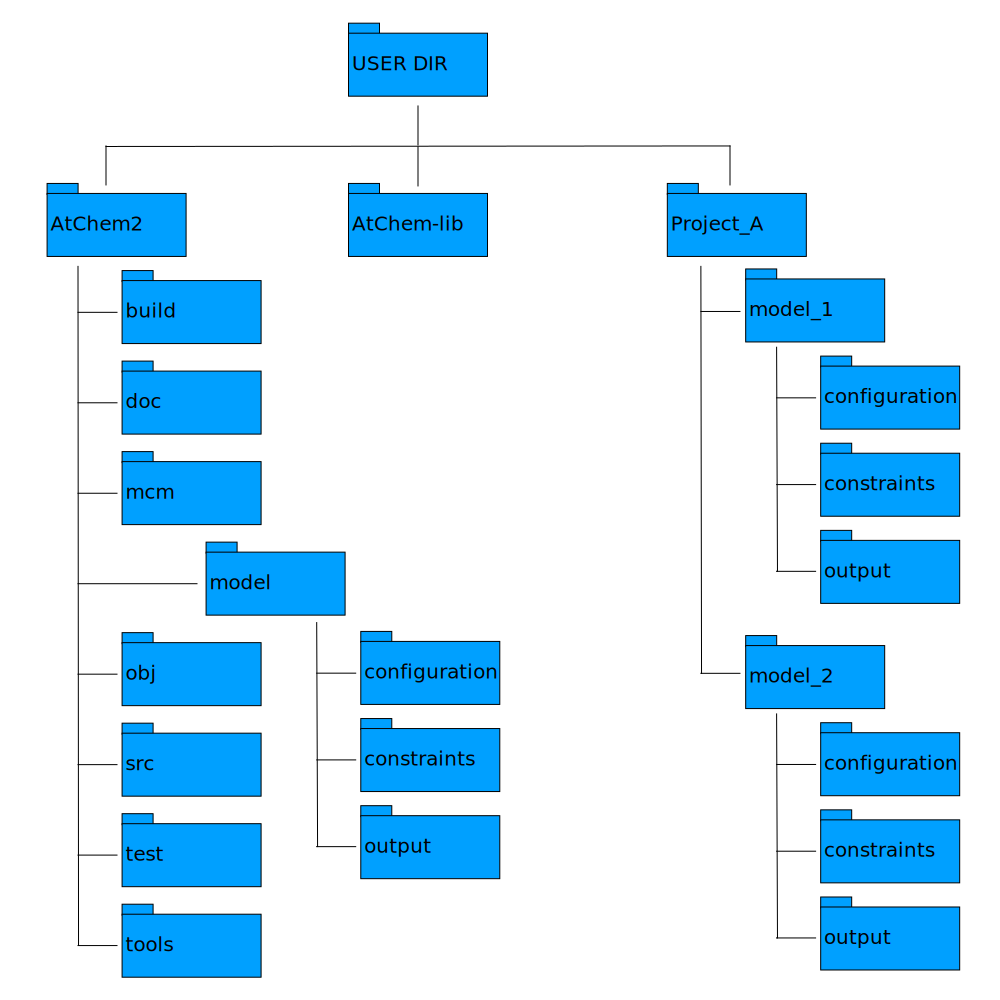
\includegraphics[width=0.85\textwidth]{model-setup.png}
  \caption{Example of a modelling setup, with an AtChem2 installation
    and a project directory containing two different box-models.}
  \label{fig:setup}
\end{figure}

Fig.~\ref{fig:setup} shows an example of a possible setup: a user
directory contains an AtChem2 installation, consisting of the
\maindir\ (\texttt{AtChem2/}, which includes the default
\texttt{model/} directory) and the \depdir\ (\texttt{AtChem-lib/}). In
addition, a project directory (\texttt{Project\_A/}) contains two
separate model directories (\texttt{model\_1/} and
\texttt{model\_2/}), each with their own chemical mechanism,
configuration, constraints and output. The project directory may
correspond, for example, to a field campaign or to a set of related
experiments. In this case, each model can be built from the \maindir\
with the following commands~\footnote{The third argument is not
  specified in this example, so the default value (\texttt{./mcm/}) is
  implicitly used.}:

\begin{verbatim}
./build/build_atchem2.sh ../Project_A/model_1/mechanism.fac
                         ../Project_A/model_1/configuration/
\end{verbatim}

\begin{verbatim}
./build/build_atchem2.sh ../Project_A/model_2/mechanism.fac
                         ../Project_A/model_2/configuration/
\end{verbatim}

There are many different ways in which the \texttt{model/} directory
can be organized and customized: for example, it is possible to keep
all the constraint files related to a project in one directory, thus
avoiding the need to have identical \texttt{constraints/} directories
in each \texttt{model/} directory. Each user has specific needs and
personal preferences; as long as the correct paths are passed to the
\texttt{build\_atchem2.sh} script (and to the executable, see
Sect.~\ref{sec:execute}), the model will compile and run.

The \texttt{build\_atchem2.sh} script also handles model compilation,
converting the Fortran code into the \texttt{atchem2} executable,
which is dynamically linked to the shared chemical mechanism library
(\texttt{mechanism.so}). If the Fortran code is not changed,
compilation is required only once for a given \texttt{.fac} (or
\texttt{.kpp}) file.

Changes to the configuration files do not require recompiling the
model. Likewise, if constraints files are added, removed or modified
there is no need to recompile the model. This is because the model
configuration and constraints are read by the executable at
runtime. However, if the chemical mechanism is changed, then the
shared library (\texttt{mechanism.so}) needs to be recompiled.
However, if the user wants, or needs, to change the Fortran code
(\texttt{src/*.f90}), then the executable needs to be recompiled.

To recompile the model, the \texttt{build\_atchem2.sh} script needs to
be executed again~\footnote{If the recompilation fails, it is
  sometimes useful to run the command \texttt{make clean} from the
  \maindir\ before rerunning the build script.}. The build script is
able to detect whether the Fortran code, the chemical mechanism, or
both have been modified, and runs the appropriate commands. This
design approach reduces both the frequency and the duration of model
compilations by requesting it only when strictly necessary, therefore
facilitating running the model in batch mode -- e.g., for sensitivity
studies.

% -------------------------------------------------------------------- %
\section{Execute} \label{sec:execute}

The build process -- described in Sect.~\ref{subsec:build-process} and
Sect.~\ref{sec:build} -- creates an executable file called
\texttt{atchem2} in the \maindir. The executable takes up to nine
arguments, corresponding to the \emph{relative paths} (with respect to
the \maindir) of the model configuration, the chemical mechanism
shared library, the constraint data files, and the model output. The
arguments are passed to the executable via a series of input
flags~\footnote{Prior to version 1.2, AtChem2 used a system of
  positional arguments instead of the input flags -- see the
  \href{https://github.com/AtChem/AtChem2/wiki/How-to-run-AtChem2}{wiki}
  for details.}, each with a default value as described below:

\begin{enumerate}
\item path to the model directory\\
  flag: \texttt{--model}\\
  default: \texttt{model/}
\item path to the directory for the model output\\
 flag: \texttt{--output}\\
 default: \texttt{model/output/}
\item path to the directory with the configuration files\\
  flag: \texttt{--configuration}\\
  default: \texttt{model/configuration/}
\item path to the directory with the model constraints\\
  flag: \texttt{--constraints}\\
  default: \texttt{model/constraints/}
\item path to the directory with the data files of constrained environment variables\\
  flag: \texttt{--env\_constraints}\\
  default: \texttt{model/constraints/environment/}
\item path to the directory with the data files of constrained photolysis rates\\
  flag: \texttt{--photo\_constraints}\\
  default: \texttt{model/constraints/photolysis/}
\item path to the directory with the data files of constrained chemical species\\
  flag: \texttt{--spec\_constraints}\\
  default: \texttt{model/constraints/species/}
\item the path to the pre-compiled chemical mechanism shared library\\
  flag: \texttt{--shared\_lib}\\
  default: \texttt{model/configuration/mechanism.so}
\item path to the directory with the MCM data files\\
  flag: \texttt{--mcm}\\
  default: \texttt{mcm/}
\end{enumerate}

In addition, the input flag \texttt{--help} displays an help message
explaining the usage of the command line arguments and of the input
flags.

AtChem2 can be run simply by executing the command \verb|./atchem2|
from the \maindir, in which case the executable will assume that all
arguments have the default values. The equivalent command using the
input flags explicitily is:

\begin{verbatim}
./atchem2 --model=model/
          --output=model/output/
          --configuration=model/configuration/
          --constraints=model/constraints/
          --spec_constraints=model/constraints/species/
          --env_constraints=model/constraints/environment/
          --photo_constraints=model/constraints/photolysis/
          --shared_lib=model/configuration/mechanism.so
          --mcm=mcm/
\end{verbatim}

Not all flags have to be used, and the order in which they are used
does not matter. If a flag is omitted, the executable assumes the
default value, based on a \emph{hierarchical directory structure}. For
example, the following command implies that a directory called
\texttt{output/} is present inside the \texttt{model/} directory, and
that three directories called \texttt{species/}, \texttt{environment/}
and \texttt{photolysis/} are present inside the
\texttt{model/constraints/} directory:

\begin{verbatim}
./atchem2 --model=model/
          --configuration=model/configuration/
          --constraints=model/constraints/
          --shared_lib=model/configuration/mechanism.so
\end{verbatim}

This approach gives the the user a lot of flexibility in the
organization of the modelling work and makes it possible to run
several models using the same executable with different
configurations, constraints and chemical mechanisms. For example, the
following commands run two models with the same chemical mechanism and
two different configurations, and save the corresponding outputs in
separate directories:

\begin{verbatim}
./atchem2 --configuration=model/configuration_1/
          --output=model/output_1/
          --shared_lib=model/mechanism.so
\end{verbatim}

\begin{verbatim}
./atchem2 --configuration=model/configuration_2/
          --output=model/output_2/
          --shared_lib=model/mechanism.so
\end{verbatim}

Only three input flags are specified in the above commands, and
therefore the executable assumes that the default values for the
remaining input flags apply -- i.e. the model directory is
\texttt{model/} and the constraints directory is the same for both
model runs (\texttt{model/constraints/}.

It is also possible to combine chemical mechanisms, configurations and
constraints from different models: for example, based on the setup
shown in Fig.~\ref{fig:setup}, the following command runs a model that
has its own configuration, but is constrained to the chemical species
and environment variables of \texttt{model\_1/} and to the photolysis
rates of \texttt{model\_2/}:

\begin{verbatim}
./atchem2 --configuration=model/configuration/
          --output=model/output/
          --shared_lib=model/configuration/mechanism.so
          --spec_constraints=../Project_A/model_1/constraints/species/
          --env_constraints=../Project_A/model_1/constraints/environment/
          --photo_constraints=../Project_A/model_2/constraints/photolysis/
\end{verbatim}

While the model is running, diagnostic information is printed to the
terminal. A successful model run completes with a message similar to
the one shown in Sect.~\ref{sec:install}. Users have the option to
redirect the terminal printout to a log file, using standard unix
commands.

\subsection{HPC} \label{subsec:hpc}

AtChem2 can be installed and run on High Performance Computing (HPC)
clusters, or supercomputers, which typically run some version of
Linux/Unix. This is recommended, especially for models with long
runtimes and/or many constraints.

Installation and setup on an HPC system are exactly the same as on a
regular workstation, but each system has its own rules and
guidelines. Therefore, it is not possible to give specific advice, and
users should check the local documentation or ask the system
administrator.

On most HPC systems, software execution is managed by a job scheduler,
which requires a submission script. The script will allocate the
requested resources~\footnote{AtChem2 does not support parallelization
  at present; this may change in future versions.}, alert the user
that the model run is finished, and save the terminal printout and any
other message to log files. The syntax and format of the submission
script depend on the type of job scheduler installed on the HPC
system. Examples of submission scripts can be found on the
\href{https://github.com/AtChem/AtChem2/wiki/Running-on-HPC}{wiki}.

% -------------------------------------------------------------------- %
\section{Output} \label{sec:output}

The model output is saved by default in the \texttt{model/output/}
directory. The location can be modified by changing the arguments of
the \texttt{atchem2} executable, as explained in Sect.~\ref{sec:execute}
(see also Sect.~\ref{subsec:model-directory}). The frequency of the model
output is determined by the following model parameters, which are set
in the \texttt{model.parameters} file (Sect.~\ref{sec:model-parameters}):

\begin{itemize}
\item \textbf{step size} for the chemical species, environment
  variables, photolysis rates and diagnostic variables.
\item \textbf{rates output step size} for the rate of production and
  destruction analysis of selected species (Sect.~\ref{subsec:ropa-roda}).
\item \textbf{reaction rates output step size} for the reaction rates
  of all chemical reactions.
\end{itemize}

All AtChem2 output files are space-delimited text files with a one
line header containing the names of the variables. The first column of
each file is the model time (\texttt{t}) in seconds since midnight of
the \textbf{start date}~\footnote{Note that the \textbf{start date} is
  different than the \textbf{model start time}. The model start time
  indicates when the model begins its run and is in seconds since the
  midnight of the start date (Sect.~\ref{sec:model-parameters}).}:

\begin{itemize}
\item Environment variables and \cf{RO2} sum:\\
  \texttt{environmentVariables.output}
\item Concentrations of selected chemical species -- see
  Sect.~\ref{subsec:outputspecies}:\\
  \texttt{speciesConcentrations.output}
\item Photolysis rates:\\
  \texttt{photolysisRates.output}
\item Latitude, longitude, solar angles and related parameters:\\
  \texttt{photolysisRatesParameters.output}
\item Loss and production rates (ROPA/RODA) of selected chemical
  species -- see Sect.~\ref{subsec:outputrates}:\\
  \texttt{lossRates.output}, \texttt{productionRates.output}
\item Concentrations of all chemical species, except the \cf{RO2} sum,
  at the end of the model run (\textbf{model stop time}):\\
  \texttt{finalModelState.output}
\item Jacobian matrix (optional, see Sect.~\ref{sec:model-parameters}):\\
  \texttt{jacobian.output}
\item Error messages and diagnostic variables:\\
  \texttt{errors.output}, \texttt{mainSolverParameters.output}
\end{itemize}

In addition to the \texttt{.output} files, the reaction rates of every
reaction in the chemical mechanism are saved, by default, in the
\texttt{output/reactionRates/} directory~\footnote{Called
  \texttt{instantaneousRates/} prior to version 1.1.}: one file for
each model step, with the name of the file corresponding to the output
time in seconds. The files have no header, and the order of reactionn
is the same as in the chemical mechanism (under the ``Reaction
definitions'' section -- see Sect.~\ref{subsec:facsimile-format}).

\subsection{ROPA/RODA} \label{subsec:ropa-roda}

The reaction rates files in the \texttt{output/reactionRates/}
directory are useful to analyze the model results and understand the
chemical system, as well as for diagnostic purposes. The format,
however, may be cumbersome to process for some users. To simplify the
rate of production and destruction analysis for specific chemical
species (i.e. those listed in \texttt{outputRates.config},
Sect.~\ref{subsec:outputrates}) AtChem2 creates the two files
\texttt{productionRates.output} and \texttt{lossRates.output}.
These files contain the reaction rates of production and destruction
of the selected species in a human-readable format, shown in
Fig.~\ref{fig:ropa}.

\begin{figure}[htb]
  \centering
  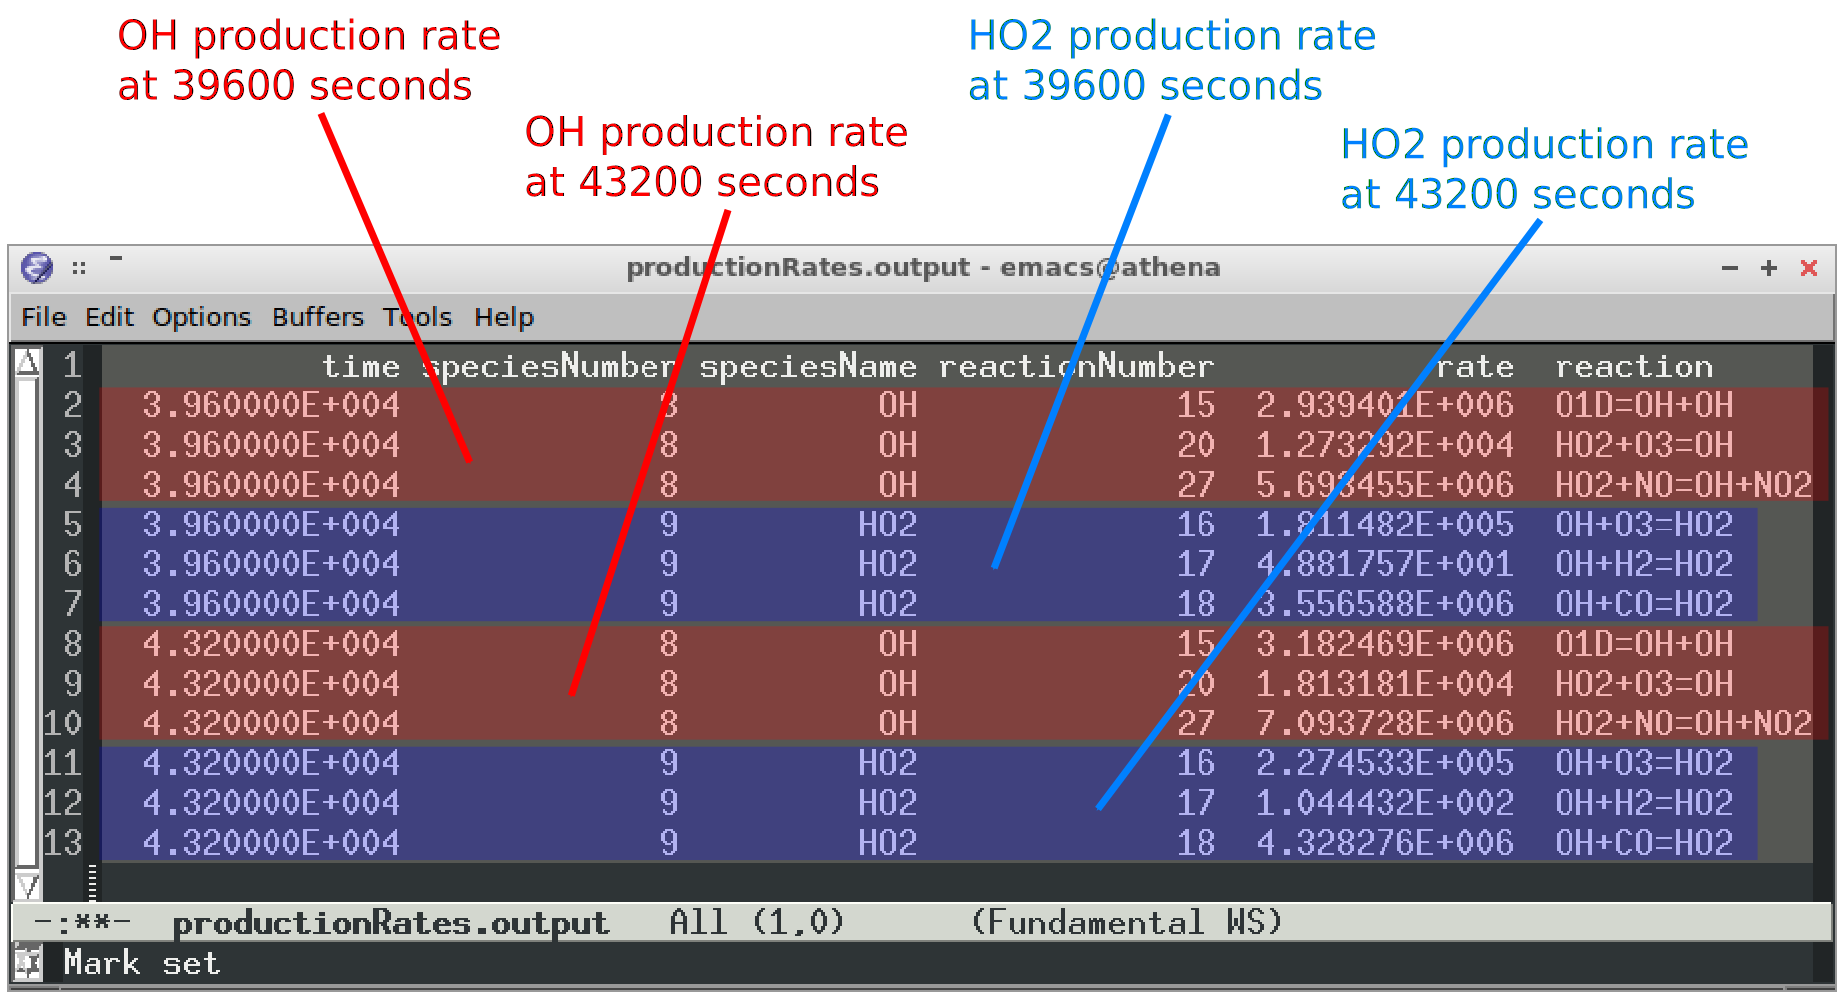
\includegraphics[width=0.95\textwidth]{output-rates.png}
  \caption{Format of the \texttt{productionRates.output} file. The
    \texttt{lossRates.output} file has a similar format.}
  \label{fig:ropa}
\end{figure}

The frequency of the ROPA/RODA output is controlled by the
parameter \textbf{rates output step size}, as explained in
Sect.~\ref{sec:model-parameters} and \ref{subsec:outputrates}. The
\texttt{productionRates.output} and \texttt{lossRates.output} files
can be very large and complex, especially for species that are
involved in many reactions and/or for long model runtimes. Therefore,
it is recommended to limit the list of chemical species in
\texttt{outputRates.config} to only those of special interest, and to
keep the frequency of the output low (the default is 1 hour).\\

\textcolor{red}{\bf Important Note}: although, in principle, a rate of
production and destruction analysis for constrained chemical species
can be done, the results should be interpreted with extreme
caution. The user must be aware that the concentrations of these
species are determined by the constraining data rather than by the
chemical reactions.
